% analysis.tex -- Section 5: Analysis
% Experiment IDs (provenance):
%   Attention entropy analysis:     attention_entropy_analysis
%   Single-step action error:       offline_singlestep_action_error
%   Action divergence:              action_divergence_v2_clean
%   Importance margin (G1):         mvp_imm_v8b_twostage
%   Token importance (G3, Spearman): plan_009_token_importance

\section{Analysis}
\label{sec:analysis}

Section~\ref{sec:results} established that all pruning configurations produce 0\% SR.
This section investigates \emph{why} the cliff edge occurs.
We present three complementary lines of evidence: the LLM backbone attends to vision tokens near-uniformly (\S\ref{sec:uniform_attention}), pruning causes immediate single-step action failures rather than gradual error accumulation (\S\ref{sec:action_disruption}), and standard offline evaluation metrics fail to predict this catastrophic closed-loop collapse (\S\ref{sec:metric_disconnect}).
Section~\ref{sec:why_vit_works} synthesizes these findings into a unified mechanistic explanation.

\subsection{Uniform Attention Distribution}
\label{sec:uniform_attention}

Token pruning in ViT classifiers succeeds because attention concentrates on a small set of discriminative patches and leaves most tokens redundant.
DynamicViT~\cite{rao2021dynamicvit} and ToMe~\cite{bolya2023tome} exploit this concentration: tokens that receive low attention contribute little to the classification decision and can be safely removed.
We test whether VLA models exhibit the same attention pattern.

We extract attention weights from the LLM backbone (Qwen2-0.5B~\cite{yang2024qwen2}) over all vision tokens across three LIBERO tasks.
The attention entropy ratio reaches 0.98 (observed entropy of 6.86 bits out of a maximum of 7.0 bits for a perfectly uniform distribution).
The two camera views receive comparable attention (53.8\% for cam1, 46.2\% for cam2), and this pattern holds across all sampled tasks with entropy values between 6.844 and 6.846 bits.
The Gini coefficient of the attention distribution is 0.246, a value that confirms low inequality across tokens.
Figure~\ref{fig:attention_heatmap} visualizes this contrast.

The architectural explanation is straightforward.
SigLIP~\cite{zhai2023siglip} encodes images using non-overlapping spatial patches without a \texttt{[CLS]} aggregation token.
Each vision token therefore corresponds to a unique spatial region of the input image, and no two tokens encode the same information.
The VLA policy must predict precise continuous actions conditioned on the full spatial layout of the scene, so the LLM backbone attends broadly to recover the complete spatial context.
This stands in direct contrast to ViT classifiers, where a single discrete label can be derived from a subset of discriminative patches and the remaining tokens contribute marginal information.

The practical consequence is clear: when attention is uniform, no subset of tokens is dispensable.
Removing any group of vision tokens removes irreplaceable spatial information from the input, regardless of how those tokens are selected.

\begin{figure}[t]
\centering
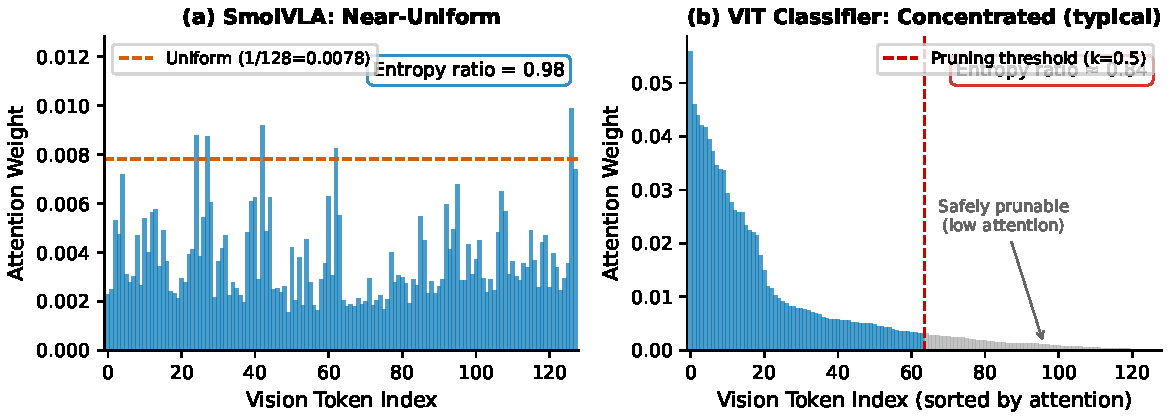
\includegraphics[width=\linewidth]{figures/paper/fig_attention_heatmap.pdf}
\caption{(a)~LLM attention over vision tokens in the VLA policy. The distribution is near-uniform (entropy ratio 0.98), with both camera views receiving comparable weight. (b)~Typical attention pattern in a ViT classifier (illustrative), where attention concentrates on a small set of discriminative patches. This concentration enables safe token pruning in classification but is absent in VLA action prediction.}
\label{fig:attention_heatmap}
\end{figure}

\subsection{Instantaneous Action Disruption}
\label{sec:action_disruption}

A natural hypothesis for the cliff edge is that small per-step errors compound over a long trajectory and eventually cause task failure.
We test this hypothesis by measuring single-step action errors under pruning, using the same observations and model checkpoint.

The results rule out gradual error accumulation.
Under the baseline (bypass mode, no pruning), the single-step L2 distance between predicted and ground-truth actions is 0.414.
Under pruning at $k{=}0.5$, this distance increases to 1.391, a 3.4$\times$ degradation.
The per-step relative error is 111.5\%; the error exceeds the magnitude of the action itself.
The failure is most severe in the gripper dimension, where the error of 1.02 indicates complete inversion: the policy commands the gripper to open when it should close, or vice versa.
Position dimensions show errors of [0.20, 0.25, 0.30] and rotation dimensions show errors of [0.01, 0.02, 0.01].

This is not a case where small errors compound into eventual failure.
A single pruned observation already produces a qualitatively wrong action.
The gripper inversion alone would cause immediate task failure in any manipulation task, independent of all subsequent steps.
Closed-loop trajectory analysis confirms this interpretation: the L2 divergence between pruned and baseline trajectories has a mean of 1.117, with onset at step~0.
The pruned policy diverges from the functional trajectory immediately, not after an accumulation period.
Figure~\ref{fig:action_divergence} shows the divergence curves.

These single-step measurements provide a direct causal link between vision token removal and action failure.
The cliff edge does not require temporal accumulation; it is instantaneous.

\begin{figure}[t]
\centering
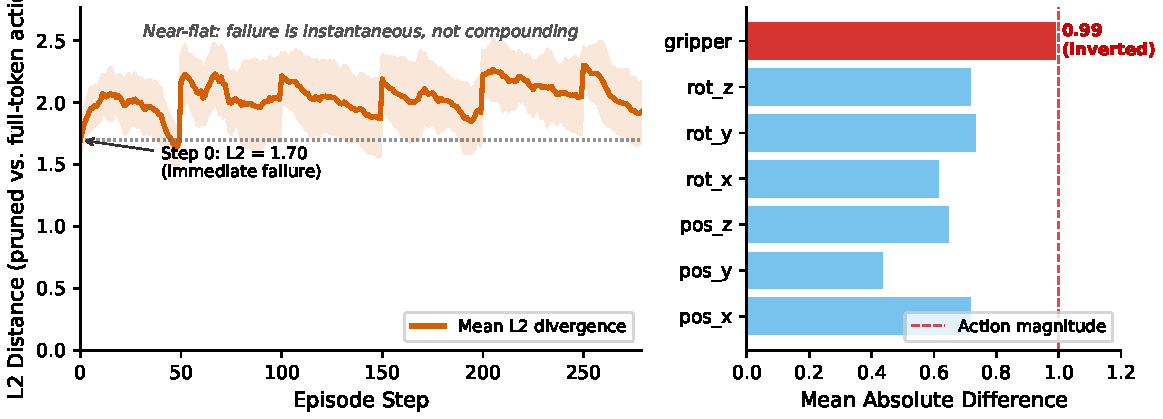
\includegraphics[width=\linewidth]{figures/paper/fig_action_divergence.pdf}
\caption{Trajectory divergence between pruned and baseline policies. The L2 distance is large from step~0 and remains elevated throughout the episode. The failure is instantaneous rather than the result of gradual error accumulation.}
\label{fig:action_divergence}
\end{figure}

\subsection{Offline Metric Disconnect}
\label{sec:metric_disconnect}

Standard practice in token pruning research is to validate a scoring function using offline metrics before deployment.
Our offline metrics provide consistently positive signals.
The importance margin gain (G1) shows a 93$\times$ improvement over the baseline, which indicates that the Attention-weighted Cumulative Importance Score (ACIS) learns to produce well-separated importance rankings.
The action loss ratio (G3) of 0.87 confirms that, on the training data distribution, the model's action loss with pruning is only 87\% of the full-token loss.
The Spearman correlation between ACIS scores and gradient magnitudes is 0.41, a moderate agreement between the learned importance scores and the gradient-based ground truth.

\begin{table}[t]
\centering
\caption{Offline evaluation metrics versus closed-loop performance. Offline ranking and loss metrics show positive signals, yet all pruning conditions produce 0\% closed-loop SR. The disconnect demonstrates that standard offline proxies are insufficient for validating VLA token compression.}
\label{tab:offline_vs_closedloop}
\small
\begin{tabular}{@{}lccr@{}}
\toprule
Metric & Result & Interpretation & SR (\%) \\
\midrule
Importance margin (G1) & 93$\times$ & Meaningful ranking & -- \\
Action loss ratio (G3) & 0.87 & Pruned $<$ full on train data & -- \\
ACIS-gradient Spearman & 0.41 & Moderate correlation & -- \\
\midrule
Single-step L2 (pruned) & 1.391 & 3.4$\times$ degradation & 0.0 \\
Relative action error & 111.5\% & Error $>$ action magnitude & 0.0 \\
Gripper error & 1.02 & Complete inversion & 0.0 \\
\bottomrule
\end{tabular}
\end{table}

Yet when pruning is actually applied, single-step action error is catastrophic: L2 of 1.391, relative error of 111.5\%, and complete gripper inversion (Table~\ref{tab:offline_vs_closedloop}).
The disconnect has a specific cause.
Ranking metrics (G1, Spearman) evaluate the quality of the importance ordering, not the effect of removing the lowest-ranked tokens.
A scorer can produce a perfect ranking yet still fail if every token carries critical information, because even the least important token may be indispensable for accurate action prediction.
The action loss ratio (G3) averages over the training set and masks the worst-case per-step errors that determine closed-loop success.
A ratio of 0.87 means the average loss increases by only 13\%, but the per-step relative error of 111.5\% reveals that the distribution of errors is heavy-tailed: the worst steps are far worse than the average suggests.

The failure cascade is consistent across all evaluation levels.
Offline ranking appears reasonable, offline action error is catastrophic, and closed-loop SR is 0\%.
This ordering implies that standard offline proxies (importance margins, averaged action losses, correlation coefficients) are necessary conditions for a good scorer but provide no guarantee of closed-loop viability.
Validating VLA compression requires closed-loop evaluation; offline metrics alone are insufficient.

\subsection{Why ViT Pruning Works but VLA Pruning Fails}
\label{sec:why_vit_works}

The three preceding analyses converge on a unified mechanistic explanation for the cliff edge.
The explanation rests on a fundamental difference between how ViT classifiers and VLA policies consume visual information.

In ViT classification, attention concentrates on a small subset of discriminative patches~\cite{rao2021dynamicvit,bolya2023tome,liang2022evit}.
The classification task requires a single discrete label from pooled features, so spatial completeness is not necessary.
Tokens outside the discriminative region carry redundant or irrelevant information, and their removal produces graceful degradation: accuracy decreases smoothly as more tokens are pruned, with less than 1\% loss even at 50\% token reduction.

In VLA action prediction, the situation is qualitatively different.
The attention distribution is near-uniform (\S\ref{sec:uniform_attention}), a direct consequence of the fact that precise continuous action prediction requires the complete spatial layout of the scene.
SigLIP~\cite{zhai2023siglip} encodes each non-overlapping spatial patch as a separate token with no \texttt{[CLS]} aggregation, so the VLA's LLM backbone must attend to all patches to reconstruct spatial relationships between the robot end-effector, target objects, and obstacles.
Removing any subset of tokens eliminates spatial information that cannot be recovered from the remaining tokens.

The consequence of this architectural difference is that the failure mode shifts from graceful degradation to binary collapse.
In classification, the error surface is smooth because the task tolerates partial spatial information.
In control, the error surface has a cliff edge because the task demands spatial completeness.
Even a 10\% token reduction ($k{=}0.9$) crosses this edge and produces 0\% SR rather than the ${\sim}$90\% that a linear degradation model would predict.

This explanation accounts for each of our empirical observations.
Uniform attention (\S\ref{sec:uniform_attention}) means no tokens are safely dispensable.
Instantaneous action disruption (\S\ref{sec:action_disruption}) means that the spatial information loss manifests as immediate qualitative failures, not subtle distributional shifts.
The offline metric disconnect (\S\ref{sec:metric_disconnect}) arises because ranking-based metrics evaluate relative importance ordering but cannot detect that all tokens exceed the criticality threshold for the downstream task.
Together, these findings indicate that token pruning as currently formulated is structurally incompatible with VLA closed-loop control, and that alternative efficiency strategies must preserve the complete vision token sequence.
